\subsubsection{Perceptrón}
Un perceptrón, o neurona es una unidad básica de inferencia en forma de discriminador lineal, es la base de lo que se conoce hoy como neurona artificial\cite{nielsen}. Básicamente, un perceptrón toma varios valores binarios como entrada $x_1, x_2, …, x_n$ y produce un único valor de salida $y$.
\newline

\begin{figure}[H]
    \centering
    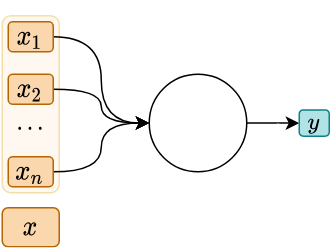
\includegraphics[width=6cm]{images/state-of-art/perceptron/perceptron.png}
    \caption{Representación del funcionamiento de un perceptrón}
    \label{fig:perceptronprocess}
\end{figure}

Además del vector $x$ y el valor $y$, el perceptron tiene dos componentes más: 
\begin{itemize}
    \item El vector de pesos $w$ que expresa la importancia de las respectivas entradas para la salida y tendrá el mismo número de elementos que $x$. Este vector se usará para calcular la suma ponderada  $\sum_i w_ix_i$.
    \item El umbral o sesgo (\textit{bias}($b$) en inglés): El valor del sumatorio se comprobará si es menor o mayor a este valor $b$. En función de ello, el valor $y$ será $0$ o $1$. El umbral es un valor que representa lo fácil que es producir un valor $1$ en $y$. Para un perceptrón con un sesgo muy grande, es extremadamente fácil que el perceptrón produzca un $1$. Pero si el sesgo es muy negativo, entonces es difícil que el perceptrón produzca un $1$.
\end{itemize}

Tanto el vector $w$ y el valor umbral $b$ son parámetros que se deben de saber previamente. El valor $y$ producido por el perceptrón viene dado por la siguiente ecuación: 

\begin{eqnarray}
  y & = & \left\{ \begin{array}{ll}
      0 & \mbox{si } \sum_i w_i x_i \leq b \\
      1 & \mbox{si } \sum_i w_i x_i > b
      \end{array} \right.
      \label{eqn:perceptroncomplex}
\end{eqnarray}


Visto gráficamente:
\begin{figure}[H]
    \centering
    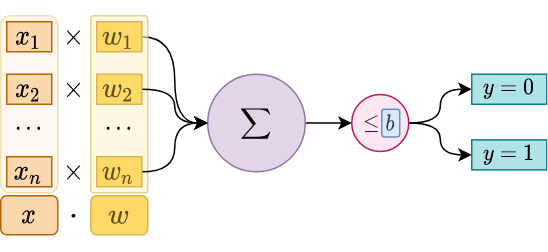
\includegraphics[width=8cm]{images/state-of-art/perceptron/perceptron_weights.png}
    \caption{Representación de un perceptrón}
    \label{fig:perceptron}
\end{figure}

Simplificando la ecuación \ref{eqn:perceptroncomplex} usando el producto vectorial y cambiando de lado $b$:
\begin{eqnarray}
  y & = & \left\{ \begin{array}{ll}
      0 & \mbox{si } w \cdot x + b \leq 0 \\
      1 & \mbox{si } w \cdot x + b > 0
      \end{array} \right.
      \label{eqn:perceptron}
\end{eqnarray}

Visto gráficamente:
\begin{figure}[H]
    \centering
    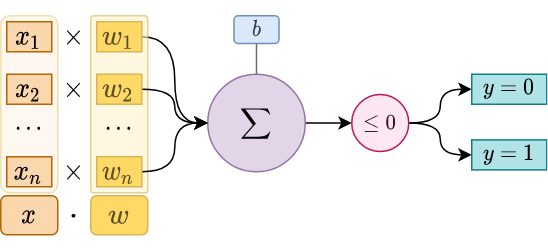
\includegraphics[width=8cm]{images/state-of-art/perceptron/perceptron_weights_complex.png}
    \caption{Representación de un perceptrón}
    \label{fig:perceptron}
\end{figure}


Los perceptrones se pueden agrupar formando capas y estas capas se pueden agrupar a su vez formando una red. Se puede ver el funcionamiento de una red neuronal programando una puerta lógica XOR que recibe dos argumentos binarios de entrada y emite una salida como se puede ver a continuación:
\begin{table}[H]
\centering
\begin{tabular}{| c | c | c |}
\hline
A & B & Salida \\
\hline
$x_1$ & $x_2$ & $y$ \\
\hline
0 & 0 & 0 \\
0 & 1 & 1\\
1 & 0 & 1\\
1 & 1 & 0\\
\hline
\end{tabular}
\caption{Puerta lógica XOR}
\end{table}

Una red neuronal que actúa como una puerta XOR es la siguiente:
\begin{figure}[H]
    \centering
    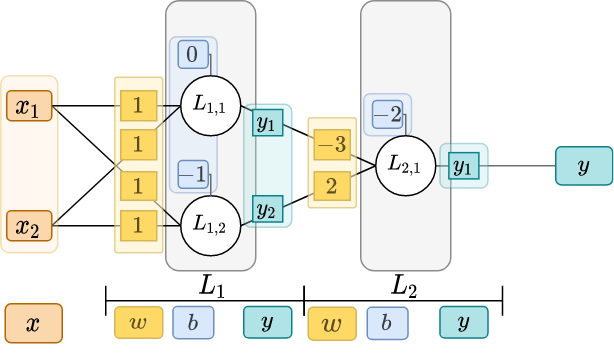
\includegraphics[width=11cm]{images/state-of-art/perceptron/xor.png}
    \caption{Red de perceptrones programada para una puerta lógica XOR}
    \label{fig:xorgatenetwork}
\end{figure}

Las redes se suelen representar con un grafo ponderado unidireccional. El grafo está dividido por capas, en este caso en dos capas ($L_1$ y $L_2$). Cada capa tiene como mínimo una neurona, que será representada por $L_{l,i}$ siendo $l$ el número de la capa e $i$ el índice de la neurona dentro de la capa. 
\newline

Los valores de los pesos se representan como si fuesen los pesos de las aristas. La cantidad de pesos que tendrá una capa asociada a ella viene dada por la multiplicación del número de neuronas en la capa $L_{l}$ por el número de neuronas en la capa anterior $L_{l-1}$. Por último, cada neurona tendrá asociado un valor $b$ que será representado como un término independiente conectado a la neurona por una línea. Por ejemplo, la neurona $L_{2,1}$ tiene asociado el vector $w = [3, -2]$ y el valor $b = -2$.
\newline

Con el grafo ya explicado, se resuelve a continuación el problema que se había planteado: Programar una puerta lógica XOR con una red neuronal. Esta red recibe recibe dos valores binarios de entrada y devolverá un único valor binario. A modo de ejemplo se realizan los cálculos para distintos ejemplos:
\begin{eqnarray}
    Para &\boxed{x = (0, 0)} \nonumber\\
    y^{L_{1,1}} & \implies & \begin{pmatrix}1&1\end{pmatrix} \cdot x^T + 0 = 0 \implies y^{L_{1,1}} = 0 \nonumber\\
    y^{L_{1,2}} & \implies &\begin{pmatrix}1&1\end{pmatrix} \cdot x^T - 1 = -1 \implies y^{L_{1,2}} = 0 \nonumber \\
    y = y^{L_{2,1}} & \implies &\begin{pmatrix}3&-2\end{pmatrix} \cdot \begin{pmatrix}0\\0\end{pmatrix} - 2= -2 \implies \boxed{y = 0} \nonumber \\ \nonumber \\
    Para &\boxed{x = (0, 1)} \nonumber\\
    y^{L_{1,1}} & \implies &\begin{pmatrix}1&1\end{pmatrix} \cdot x^T + 0 = 1 \implies y^{L_{1,1}} = 1\nonumber\\
    y^{L_{1,2}} & \implies &\begin{pmatrix}1&1 \end{pmatrix} \cdot x^T - 1 = 0 \implies y^{L_{1,2}} = 0\nonumber\\
    y = y^{L_{2,1}} & \implies &\begin{pmatrix}3&-2\end{pmatrix} \cdot \begin{pmatrix}1\\0\end{pmatrix} - 2 = 1 \implies \boxed{y = 1}\nonumber \\ \nonumber \\
    Para &\boxed{x = (1, 1)} \nonumber\\
    y^{L_{1,1}} & \implies &\begin{pmatrix}1&1\end{pmatrix} \cdot x^T + 0 = 2 \implies y^{L_{1,1}} = 1\nonumber\\
    y^{L_{1,2}} & \implies &\begin{pmatrix}1&1 \end{pmatrix} \cdot x^T - 1 = 1 \implies y^{L_{1,2}} = 1\nonumber\\
    y = y^{L_{2,1}} & \implies &\begin{pmatrix}3&-2\end{pmatrix} \cdot \begin{pmatrix}1\\1\end{pmatrix} - 2 = -1 \implies \boxed{y = 0}\nonumber \\ \nonumber
\end{eqnarray}
